\section*{Appendix II - Gabor and Morlet Wavelets}
\subsection*{Gabor Wavelet filter}
The 1D-Gabor wavelet is defined spatially by
\begin{equation}
    \psi(x)=exp\left(-\frac{x^2}{2\sigma^2}+i\xi x\right)
    \label{eqn_app2_wfil00}
\end{equation}
The Fourier-transform is
\begin{equation}
    \hat{\psi}(\omega)=exp\left(-\frac{\sigma^2(\omega-\xi)^2}{2}\right)
    \label{eqn_app2_wfil01}
\end{equation}
It's value bounded at 0 is $\hat{\psi(0)}=exp(-\sigma^2\xi^2/2)$, so we have
\begin{equation}
    \xi\sigma=\sqrt{-2\log(\hat{\xi}(0))}
    \label{eqn_app2_wfil02}
\end{equation}
The wavelets are therefore computed as 
\begin{equation}
    \psi_j=\frac{1}{a^j\sigma}\left(\frac{x}{a^j}\right)
    \label{eqn_app2_wfil03}
\end{equation}

Where $a$ is the scale factor.  if we call $\tau$, the value of the two Gabor where the plots intersect, we have, as in figure \ref{fig_app2_gab}.
\begin{figure}
\centering
  % Requires \usepackage{graphicx}
  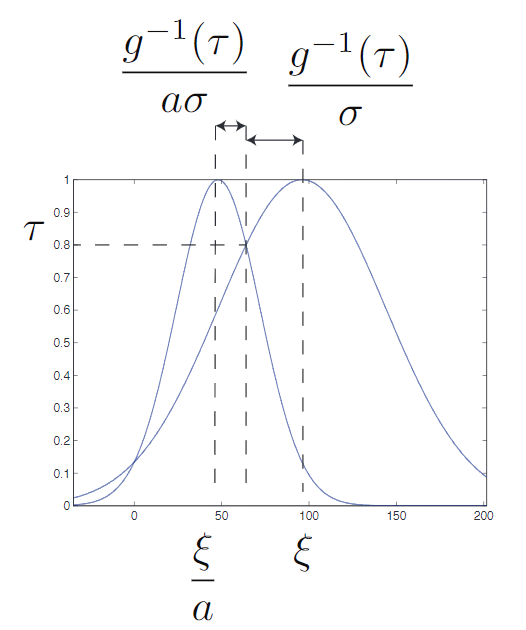
\includegraphics[width=14cm]{thesis/images/gab}\\
  \caption{Two-Gabor Plots showing $\tau$} \label{fig_app2_gab}
\end{figure}